\chapter{Lo Strato Applicativo: DNS}
\section{Introduzione}

Ogni rete e' identificata sulla rete tramite un indirizzo IP.
Il problema di essi e' che non sono facili da ricordare \textit{\tiny e sono brutti}.
E' quindi nato il bisogno di associare gli IP a dei nomi logici (e spesso mnemonici).
Per associare gli IP ai nomi e' stato creato il DNS.

Il DNS adotta il paradigma client-server.
Si affida al protocollo di trasporto sottostante per trasferire i messaggi.
E' costituito da:
\begin{itemize}
    \item Uno schema di assegnazione dei nomi
    \item Un database distribuito contenente le associazioni 
    \begin{center}
        $nome dominio \implies IP$
    \end{center}
    \item Un protocollo per la distribuzione delle informazioni sui nomi tra i name server
    \begin{itemize}
        \item Utilizza UDP (porta 53) [oppure TCP]
    \end{itemize}
\end{itemize}

\section{Servizi DNS}
\paragraph{Risoluzione} Traduzione $hostname \implies indirizzo IP$
\paragraph{Host aliasing} Traduzione $nomi \implies nome canonico / IP$
\paragraph{Mail server aliasing} Stessa cosa degli host, permette tra le altre cose di usare nomi identici per mail e web server.
\paragraph{Distribuzione di carico} Ad un hostname possono corrispondere piu' indirizzi IP; il DNS restituisce la lista di IP variandone l'ordinamento ogni volta.
\section{Spazio dei nomi}
{\color{YellowOrange}\paragraph{Struttura "flat"} Sequenza di caratteri senza alcuna ulteriore struttura (deprecato)}
\paragraph{Struttura gerarchica} Il nome e' costituito da diverse parti
\begin{center}
    (p.e. studenti.di.unipi.it)
\end{center}
L'assegnazione dei nomi e' delegabile al sistema decentralizzato. 
\subsection{Nomi di dominio}
I nomi hanno una struttura ad albero. Ogni nodo e' individuato da un'etichetta.(la radice ha etichetta vuota)
\newline
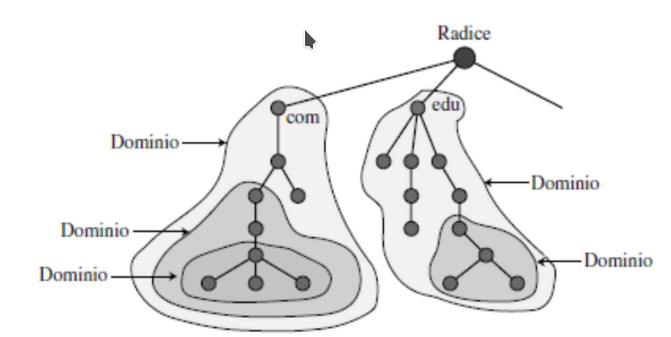
\includegraphics[width=\textwidth]{dns-tree}
La struttura gerarchica permette autonomia nella scelta dei nomi all'interno di un dominio.
\subsection{Esempi di Top Level Domain (TLD)}
\begin{description}
    \item[com] Organizzazioni commerciali
    \item[edu] Istituti di istruzione
    \item[mil] Gruppi militari
    \item[gov] Istituzioni governative
    \item[net] Centri di supporto alla rete
    \item[org] Organizzazioni diverse dalle precedenti
    \item[it, uk, fr, us] Schema geografico per nazioni  
\end{description}
Mantenuti da IANA (Internet Assigned Numbers Authority)
\section{Gerarchia dei Name Server}
\paragraph{DNS} Database distribuito implementato come gerarchia di piu' Name Server.
\paragraph{Name Server} Gestisce le richieste.
Ogni server immagazzina le informazioni relative alla propria zona inclusi i riferimenti ai server dei domini di livello inferiore.
\subsection{Root Name Server}
Restituisce le informazioni sui name server dei TLD. Ce ne sono centinaia in tutto il mondo.
\subsection{TLD Server}
Mantiene le informazioni dei nomi di dominio che appartengono a un TLD; Restituisce le informazioni sui Name Server di competenza dei sotto domini.
\subsection{Authoritative Name Server} %TODO - Non ci ho capito un cazzo
E' l'autorità per una certa zona. Puo' effettuare traduzioni nome $\implies$ indirizzo o inoltrare la richiesta a altri Name Servers.
Sono di due tipi:
\begin{description}
    \item[Server primari] Mantengono il file di zona.
    \item[Server secondari] Ricevono il file di zona e offrono il servizio di traduzione. 
\end{description}
\subsection{Local Name Server}
E' un Name Server mantenuto dagli ISP.
Le query DNS vengono prima rivolte al server locale il quale, in caso non riesca a risolverle, le inoltra alla gerarchia DNS.
\subsection{Query DNS}
La query puo' essere:
\begin{description}
    \item[Ricorsiva] La richiesta fa il \textit{giro completo} attraversando ogni name server fino a trovare il dominio che sta' cercando.
    \item[Iterativa] Le risposte sono restituite direttamente al client insieme al riferimento al server da contattare.
\end{description}
\subsection{DNS Caching}
I name server mantengono una memoria delle associazioni gia' richieste, le quali vengono cancellate dopo un tempo di timeout.
\section{Resource Records}
\begin{center}
    RR format: \textbf{(name, value, type, ttl)}
\end{center}
\begin{description}
    \item[TTL] Tempo di vita della risorsa della cache.
    \item[Type] A 
    \begin{description}
        \item[Name]  hostname
        \item[Value] IP 
    \end{description}  
    \item[Type] CNAME
    \begin{description}
        \item[Name] hostname
        \item[Value] nome canonico  
    \end{description} 
    \item[Type] NS
    \begin{description}
        \item[Name] Nome di dominio
        \item[Value] hostname dell'authoritative name server per quel dominio
    \end{description} 
    \item[Type] MX
    \begin{description}
        \item[Name] Nome di dominio
        \item[Value] Nome canonico del server di posta elettronica associato
    \end{description} 
\end{description}
% \subsection{Messaggi DNS} TODO
